% mnras_template.tex
%
% LaTeX template for creating an MNRAS paper
%
% v3.0 released 14 May 2015
% (version numbers match those of mnras.cls)
%
% Copyright (C) Royal Astronomical Society 2015
% Authors:
% Keith T. Smith (Royal Astronomical Society)

% Change log
%
% v3.0 May 2015
%    Renamed to match the new package name
%    Version number matches mnras.cls
%    A few minor tweaks to wording
% v1.0 September 2013
%    Beta testing only - never publicly released
%    First version: a simple (ish) template for creating an MNRAS paper

%%%%%%%%%%%%%%%%%%%%%%%%%%%%%%%%%%%%%%%%%%%%%%%%%%
% Basic setup. Most papers should leave these options alone.
\documentclass[fleqn,usenatbib]{mnras}

% MNRAS is set in Times font. If you don't have this installed (most LaTeX
% installations will be fine) or prefer the old Computer Modern fonts, comment
% out the following line
\usepackage{newtxtext,newtxmath}
% Depending on your LaTeX fonts installation, you might get better results with one of these:
%\usepackage{mathptmx}
%\usepackage{txfonts}

% Use vector fonts, so it zooms properly in on-screen viewing software
% Don't change these lines unless you know what you are doing
\usepackage[T1]{fontenc}
\usepackage{ae,aecompl}


%%%%% AUTHORS - PLACE YOUR OWN PACKAGES HERE %%%%%

% Only include extra packages if you really need them. Common packages are:
\usepackage{graphicx}	% Including figure files
\usepackage{amsmath}	% Advanced maths commands
\usepackage{gensymb}
\usepackage{amssymb}	% Extra maths symbols
\usepackage{color} % Colour fonts
\usepackage{subfiles} % allows defining sections in their own files
\usepackage[british]{babel}
\usepackage[utf8]{inputenc}

\selectlanguage{british}

%%%%%%%%%%%%%%%%%%%%%%%%%%%%%%%%%%%%%%%%%%%%%%%%%%

%%%%% AUTHORS - PLACE YOUR OWN COMMANDS HERE %%%%%

% Please keep new commands to a minimum, and use \newcommand not \def to avoid
% overwriting existing commands. Example:
%\newcommand{\pcm}{\,cm$^{-2}$}	% per cm-squared

\definecolor{comment}{RGB}{200,0,0}
\renewcommand{\comment}[2][comment]{{\color{#1}[[{\bf #2}]]}}

\newcommand{\widevec}[1]{\overrightarrow{#1}}
\newcommand{\Lingard}{\comment{Lingard et al. (2020)}}

%%%%%%%%%%%%%%%%%%%%%%%%%%%%%%%%%%%%%%%%%%%%%%%%%%

%%%%%%%%%%%%%%%%%%% TITLE PAGE %%%%%%%%%%%%%%%%%%%

% Title of the paper, and the short title which is used in the headers.
% Keep the title short and informative.
\title[Galaxy Zoo Builder: Morphological Dependence of Spiral galaxy pitch angle]{Galaxy Zoo Builder: Morphological Dependence of Spiral Galaxy pitch angle}

% The list of authors, and the short list which is used in the headers.
% If you need two or more lines of authors, add an extra line using \newauthor
\author[T. Lingard et al.]{
  Timothy Lingard$^{1}$\thanks{E-mail: tklingard@gmail.com},
  Karen L. Masters$^{2}$,
  Coleman Krawczyk$^{1}$,
  % Chris Lintott$^{3}$,
  % \newauthor
  % Steven Bamford,$^{4}$,
  % Sandor Kruk,$^{5}$,
  % Brooke Simmons,$^{6}$,
  % Robert Simpson,$^{7}$,
  % \newauthor
  Robert C. Nichol,$^{1}$
  \\
  % List of institutions
  $^{1}$Institute of Cosmology and Gravitation, University of Portsmouth, Dennis Sciama Building, Burnaby Road, Portsmouth, PO1 3FX, UK\\
  $^{2}$Haverford College, 370 Lancaster Ave., Haverford, PA 19041, USA\\
  % $^{3}$Oxford Astrophysics, Denys Wilkinson Building, Keble Road, Oxford, OX1 3RH, UK\\
  % $^{4}$Centre for Astronomy \& Particle Theory, School of Physics \& Astronomy, University of Nottingham, Nottingham, NG7 2RD, UK\\
  % $^{5}$European Space Agency, ESTEC, Keplerlaan 1, NL-2201 AZ, Noordwijk, The Netherlands\\
  % $^{6}$Physics Department, Lancaster University, Lancaster, LA1 4YB, UK\\
  % $^{7}$\\
}

% These dates will be filled out by the publisher
\date{Accepted XXX. Received YYY; in original form ZZZ}

% Enter the current year, for the copyright statements etc.
\pubyear{2019}

% use this if getting \pdfendlink ended up in different nesting than \pdfstartlink
\hypersetup{draft}

% Don't change these lines
\begin{document}
\label{firstpage}
\pagerange{\pageref{firstpage}--\pageref{lastpage}}
\maketitle

% Abstract of the paper
\begin{abstract}
\subfile{sections/abstract}
\end{abstract}

% Select between one and six entries from the list of approved keywords.
% Don't make up new ones.
\begin{keywords}
galaxies: evolution -- galaxies: spiral -- galaxies: photometry
\end{keywords}

%%%%%%%%%%%%%%%%%%%%%%%%%%%%%%%%%%%%%%%%%%%%%%%%%%

%%%%%%%%%%%%%%%%% BODY OF PAPER %%%%%%%%%%%%%%%%%%

% \section*{Intro Lit review (to be removed)}
% % !TEX root = ../main.tex

\citet{2014PASA...31...35D} introduction:

\begin{itemize}
  \item spirals patterns are present in 2/3 of all massive galaxies (GZ2)
  \item Sites of a majority of a star formation
  \item understanding spirals is essential for understanding star formation and galaxy evolution
  \item hubble classification of spirals are divided by tightness and the presence of a bar
  \item can also include information on bulge size and luminosity, and galaxy gas content
  \item Elmegreen \& Elmegreen proposed another scheme, classifying spirals into 12 types depending on the number and lenght of spiral arms
  \item This was simplified into \textit{flocculent}, \textit{grand design} and \textit{multi-armed} spirals
  \item 60\% of galaxies exhibit some grand design structure
  \item the type of spiral is linked to the mechanism which generated them
  \begin{itemize}
    \item (quasi-stationary) density wave theory (\textit{QSDW})
    \item local instabilities, perturbations or noise which are swing-amplified
    \item tidal interactions
    \item bars may also play a role in inducing spiral arms
  \end{itemize}
  \item \textbf{these mechanisms are not mutually exclusive}
  \item flocculent and multi-arm spirals generally thought to arise from local instabilities
  \item grand designs are thought to have undergone a tidal interaction, have a bar driving arms or be obeying \textit{QSDW}
  \item we can measure spiral number, pitch angle, amplitude, arm shape and lifetime
\end{itemize}

\citet{2019MNRAS.487.1808M} introduction:

\begin{itemize}
  \item Hubble classification is a common technique
  \item Hubble spirals are ordered in a sequence extending away from the ellipticals, and separated depending on the presence of a bar
  \item Extended by de Vaucouleurs to include Sd
  \begin{itemize}
    \item split by spiral arm appearance (how tightly wound and how distinct the arms were)
    \item the prominence of a central bulge
  \end{itemize}
  \item galaxy morphology encodes information on its dynamical history, including its formation and evolution
  \item morphology is known to correlate well with other physical properties
  \item people have taken to using proxies for morphology
  \item this is not a valid approach
  \item this paper explores an updated view of the Hubble sequence with the morphological classifications provided by Willett et al. (2013)
  \item most experts say that classifying based on bulge size vs spiral tightness result in consistent classification
  \item modern automatic galaxy classification conflates bulge size alone with spiral type
  \item differences in arm characteristics is linked to different formation mechanisms (floculent to shearing, grand design to density waves)
\end{itemize}

\citet{2019arXiv190804246D} introduction:

\begin{itemize}
  \item Arms are noticeable and pretty and they host intense star formation, H2 regions and dust.
  \item More prominent in blue, but backbone is comprised of old stars.
  \item 2/3 massive galaxies are Spirals.
  \item 3 types of spiral arm (GD, 18\%; FL, 50\%; MA, 32\%; Elmegreen et al, 2011 and Buta et al., 2015).
  \item GD have two long and well-defined spiral arms, FL have short and fragmented arm sections, MA are a fairly symmetric middle-ground, comprised of central 2-armed section which develops long ramifications in teh outer parts of the optical disc.
  \item Spiral formation is a matter of debate - including \textit{density wave theory}, \textit{tidal triggering} and \textit{swing amplification}.
  \item GD spirals and inner section of MA spirals are seen as density wave driven, whereas FL patterns are seen as swing-amplified regions of local gravitational instability
  \item Numerical models show that FL patterns are transient and reccurent, whereas GD last longer ($\sim1$ Gyr).
  \item pitch angle is a measure of arm tightness. Positive pich angle gives trailing arm, and vice versa.
  \item pitch angle is not necessarily constant, regardless of the class of the spiral arm.
  \item It is claimed that pitch angles depend on central mass concentration and atomic gas density (e.g. Kennicutt 1981; Block et al. 1994; Davis et al. 2015; Yu \& Ho 2019), galactic shear rate (e.g. Seigar et al. 2006; Grand et al. 2013), or on the steepness of the rotation curves (Seigar et al. 2005, 2014).
  \item Spiral arms are more open in galaxies with rising rotation curves (larger absolute pitch angle) and tighter in those with falling rotation curves.
  \item Very tight scaling relation reported by Davis et al. (2017) between supermassive black hole mass and the spiral pitch angle.
  \item Spirals rearrange gas and lead to the formation of disc-like bulges (e.g. Kormendy \& Kennicutt 2004). Making them important agents for the secular evolution of disc galaxies (a process in which bars also play a significant role).
  \item Spirals could be driven by bars, though this is still debated. Manifold theory suggests a strong coupling between bars and spirals (Romero-G\'omez et al. 2006, and many others). Numerical simulations show that material becomes confined to tubes (invariant manifolds) that extend from the two unstable Lagrangian points at the end of the bar ($L_1$ and $L_2$). This theory predicts a dependence of the pitch angle on the bar perturbation strength (Athanassoula et al. 2009a).
\end{itemize}

\citet{2019arXiv190910291P} introduction:

\begin{itemize}
  \item Spirals make up \textbf{one-third} (\textit{this is a typo, two-thirds is correct}) of all massive galaxies
  \item They are the site of a majority of star formation
  \item Dobbs and Baba argue that in unbarred spirals spiral arms are either transient and recurrent due to self-gravity within steller and / or gaseous discs, or are the result of tidal interactions
  \item Supported by lack of relation between pitch angle and central galaxy concentration observed in GZ (Hart 2017)
  \item Shabani et al. (2018) only find evidence of a fixed density wave in a galaxy with a strong bar, however Yu and Ho (2018, 2019) do find correlations between pitch angle and galaxy morphology
\end{itemize}

\subsection*{TL;DR}

Understanding spirals is very useful

Spiral tightness can be used as a measure of useful things

It's difficult to measure spiral tightness at scale

Bars cause predictions of tightness to change measurably


\section{Introduction}
% !TEX root = ../main.tex

Spiral structure is present in a majority of massive galaxies (e.g. \citealt{1989gadv.book..151B}, \citealt{2008MNRAS.389.1179L}) yet the formation mechanisms through which spiral structure originates are still hotly debated (e.g. \citealt{2014PASA...31...35D}). Spirals are as diverse as the theories proposed to govern their evolution, from the quintessential pair of well-defined arcs of the grand design spiral, to the fragmented arm segments of the flocculent spiral, to the disjointed multi-armed spiral.
(\citealt{2011ApJ...737...32E}; examples of each type are shown in Figure \ref{fig:spiral-galaxy-types}). The Hubble classification scheme \citep{1926ApJ....64..321H} and its revisions and expansions \citep{1961hag..book.....S,1991rc3..book.....D} contain detailed variations of different types of spiral galaxy, divided by the presence of a bar and ordered by the \textbf{openness of the spiral arms, the} degree of resolution \textbf{into condensations} and the prominence of a central bulge. Building on this, \citet{1982MNRAS.201.1021E} found that flocculent spirals are more prevalent in unbarred, isolated galaxies. The presence of a bar, a binary companion or group membership result in a higher fraction of observed grand design spiral patterns.

\begin{figure*}
  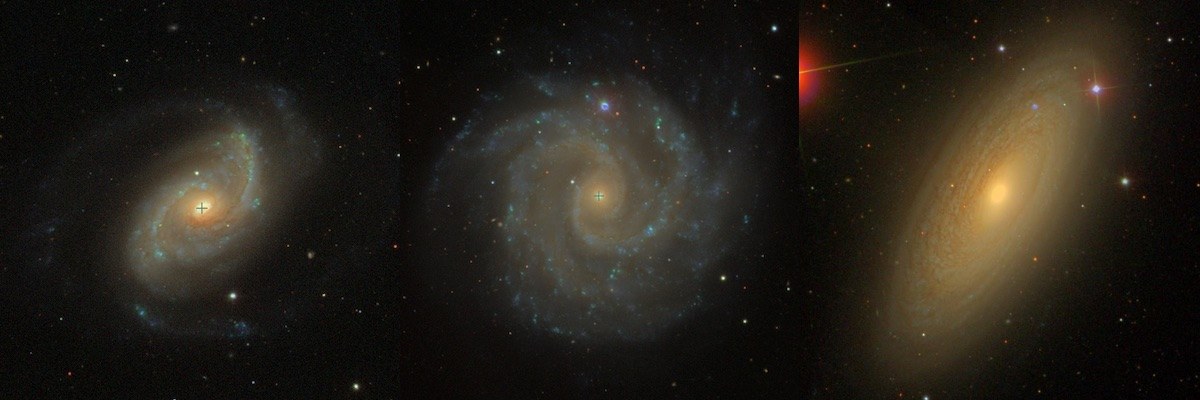
\includegraphics[width=15cm]{plots/galaxy_types_remade.jpg}
  \caption{Examples of the different types of spiral galaxy present in the sky. The left column shows the grand design spiral NGC 5248. the middle shows the many-armed spiral NGC-3184 and the right shows the flocculent spiral NGC {\bf 2841}. Images were taken with the Sloan Digital Sky Survey Telescope.}
  \label{fig:spiral-galaxy-types}
\end{figure*}

Whatever kind of spiral is present in a disc galaxy, there is plenty of evidence to suggest that they have a significant role on the overall evolution of that galaxy. For example, a majority of the population of young stars in a galaxy are located in its spiral arms \citep{2011EAS....51...19E}, and there is evidence that spiral arms may trigger star formation \citep{2013A&A...560A..59C} perhaps via their ability to promote the growth of Giant Molecular Clouds \citep{2014IAUS..298..221D}. The rearrangement of disc gas and stars driven by spiral arms (e.g. \citealt{2018MNRAS.476.1561D}) may lead to the formation of disc-like bulges (commonly called ``pseudobulges''; e.g. \citealt{2004ARA&A..42..603K}), which are prevalent in most spiral galaxies, including those without bars \citep{2010ApJ...716..942F}. Studies of spiral morphology have also found interesting correlations with other galactic properties, such as a correlation between the tightness of spiral arms and central mass concentration (\citealt{2019ApJ...871..194Y}, though neither \citealt{2017MNRAS.472.2263H} nor \citealt{2019MNRAS.487.1808M} found such a relation in large samples). Spiral tightness is also observed to correlate with with rotation curve shape (\citealt{2005MNRAS.359.1065S}), with \textbf{galaxies with rising rotation curves having} more open spiral structure. These predictions and observations provide compelling reasons for continued investigation of the underlying rules and dynamics of spiral structure, as doing so is essential for understanding the secular evolution of disc galaxies.

Our current understanding of the mechanisms which drive spiral growth and evolution suggests that different forms of spiral arms in a galaxy may be triggered by different processes. Grand design spirals are thought to have undergone a tidal interaction \citep{2010MNRAS.403..625D,2017ApJ...834....7S}, be driven by a bar (as seen in gas simulations, \citealt{1976ApJ...209...53S,2008A&A...489..115R}, and suggested for stars by Manifold theory, \citealt{2006A&A...453...39R,2009MNRAS.394...67A,2009MNRAS.400.1706A}), or be obeying (quasi-stationary) density wave theory (QSDW theory), in which spiral arms are slowly evolving, ever-present structures in the disc (as first proposed by \citealt{1964ApJ...140..646L}). Flocculent spirals are thought to be formed through swing amplification (shearing of small gravitational instabilities in the disc), and be transient and recurrent in nature \citep{1966ApJ...146..810J}.

One of the fundamental assumptions of early work on spiral formation mechanisms (primarily QSDW) was that the disc of a galaxy, if unstable to spiral perturbations, would create a stable, static wave which would exist unchanged for many rotational periods \citep{1964ApJ...140..646L}. The motivation for static waves with small numbers of arms was primarily observational: most disc galaxies observed at the time showed spiral structure with low spiral arm numbers, suggesting that spirals exist for a long time or are continually rebuilt. This, in combination with theoretical arguments about the ``winding problem", motivated the original static density waves of \citet{1964ApJ...140..646L}, to which swing amplification was added by \citet{Toomre1981}  to provide a way to counteract the short lifetime of stellar density waves.

More recently, simulations demonstrate that spirals do not maintain a constant tightness (often quantified by pitch angle, the angle between the spiral and the tangent to a circle centred on the galaxy, \citealt{1987gady.book.....B}, illustrated in Figure \ref{fig:pitch-angle-example}), and instead wind-up over time due to the differential rotation of the disc \citep{2013ApJ...763...46B}. Recent research suggests that spirals arms are transient, and continually dissipate and re-form \citep{2014PASA...31...35D}. These spirals can be maintained through the same mechanisms that drive QSDW spirals (i.e. ``wave amplification by stimulated emission of radiation'', \citealt{1976ApJ...205..363M}; swing amplification, \citealt{1965MNRAS.130..125G}), but do not require the idealistic disc conditions required for the formation and maintenance of a stationary wave. The pitch angles of these transient spiral arms will decrease due to the differential rotation of the disc, with the density of the arm peaking at some critical pitch angle, before dissipating to be reformed.

\begin{figure}
  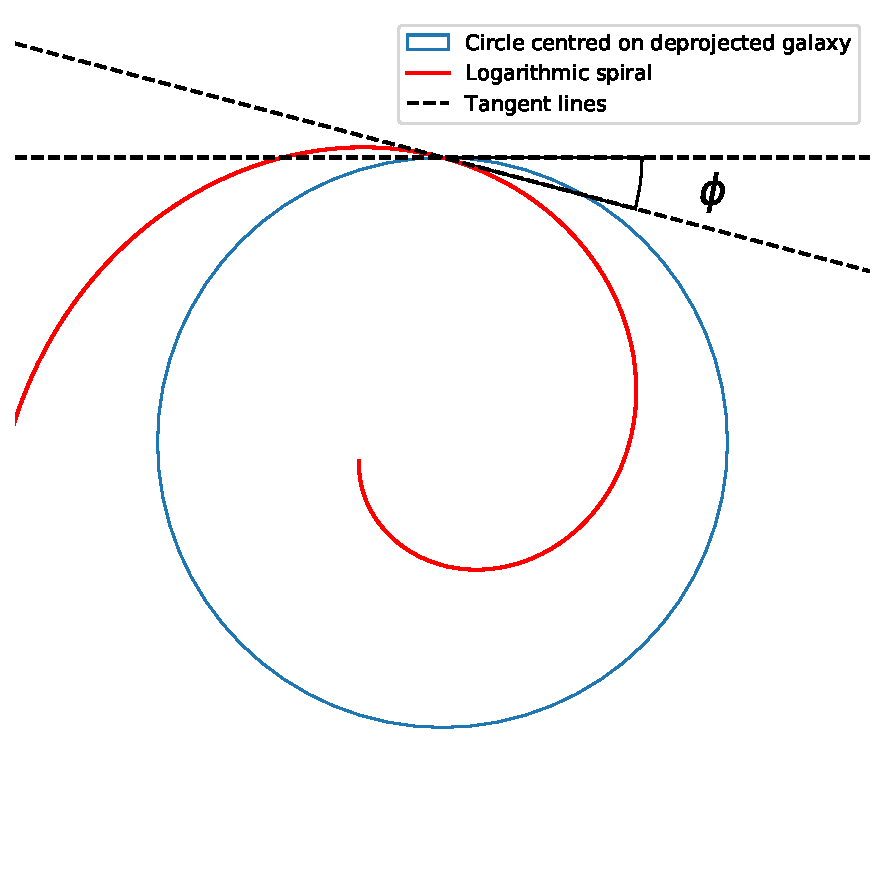
\includegraphics[width=8.4cm]{plots/pitch-angle-explanation.pdf}
  \caption{Illustration of the definition of pitch angle. It is given as $\phi = \tan^{-1}\left(\frac{\mathrm{d}r}{\mathrm{d}\theta}\ /\ r\right)$, or the angle between the spiral (red) and the tangent to a circle centred on the galaxy (blue).}
  \label{fig:pitch-angle-example}
\end{figure}

In this dynamic picture of spiral arms, pitch angle monotonically decreases from a spiral arm's formation to its dissipation. As a particular example of this, \citet{2019arXiv190910291P} propose a simple test of the winding of spiral arms, predicting that the cotangent of the pitch angle of a spiral arm ($\cot \phi$) evolves linearly with time. They found that the distribution of pitch angles of their sample of 86 galaxies was consistent with this prediction, which they present as evidence against QSDW theory in favour of the dynamic spirals produced in many simulations.

We aim to test this idea of spiral winding using data from the \textit{Galaxy Builder} citizen science project for the spiral galaxies present in \citet{2020arXiv200610450L}. We make use of Bayesian hierarchical modelling to measure galaxy pitch angle from the spiral arms produced by \textit{Galaxy Builder}. This methodology allows us to quantify the differences in pitch angles between arms in a single galaxy, as well as investigate the distribution of pitch angles in the galaxy population and investigate relationships between pitch angle and galaxy morphology.

Using Galaxy Zoo 2 data \citep{Willett2013:1308.3496v2} we further separate the galaxies by the presence and strength of a stellar bar. This will allow us to test simulations of gas in barred galaxies, which often demonstrate that bars can drive long-term spiral evolution \citep{2008A&A...489..115R}, or boost transient spiral structure \citep{2012MNRAS.426..167G}. Manifold theory \citep{2006A&A...453...39R,2009MNRAS.394...67A,2009MNRAS.400.1706A} is one attempt to determine the orbits of stars in bar-driven spiral arms: it proposes that stars in the vicinity of the unstable Lagrangian points at either end of the bar tend to escape along predictable orbits, governed by invariant manifolds. One of the primary factors influencing the shape of this invariant manifold is the relative strength of the non-axisymmetric forcing caused by the bar, with stronger bars resulting in spirals with larger pitch angles.

Many other galactic components may correlate with spiral morphology, including bulge fraction (\citealt{1975A&A....44..363Y}, \citealt{2013MNRAS.436.1074S}, \citealt{2019MNRAS.487.1808M}) and black hole mass (\citealt{2008ApJ...678L..93S}, \citealt{2017MNRAS.471.2187D}, \citealt{2019MS&E..571a2118A}). Larger bulges and more massive central black holes have both been observed to correlate with more tightly wound spiral arms. We can also test this with the data presented in this paper.

This paper is structured as follows: In Section \ref{section:method} we introduce methods to measure galaxy pitch angle, and present our sample, and our Bayesian hierarchical modelling method making use of \textit{Galaxy Builder} to estimate galaxy and population pitch angles. Section \ref{section:constraints-on-galaxy-phi} presents our general constraints on pitch angles in our section, while Section \ref{section:morphology-comparison} examines the correlation between pitch angle and bulge size implied by the Hubble sequence, and pitch angle and bar strength implied by Manifold theory. Section \ref{section:spiral_winding} investigates spiral arm winding using the test derived by \cite{2019arXiv190910291P} (uniformity of galaxy pitch angle in $\cot\;\phi$). We provide a summary and conclusions in Section \ref{section:summary}.  Where necessary, we make use of $H_0 = 70\ \text{km}\ \text{s}^{-1}\ \text{Mpc}^{-1}$.

% \newpage

\section{Method}
% !TEX root = ../main.tex
\label{section:method}

\subsection{Measuring galaxy pitch angle}
Many methodologies have been proposed and implemented to measure spiral arm properties, including visual inspection (\citealt{2015A&A...582A..86H}), Fourier analysis (i.e. \textsc{2DFFT}, \citealt{2012ApJS..199...33D}), texture analysis (i.e. SpArcFiRe, \citealt{2014ApJ...790...87D}), and combinations of automated methods and human classifiers (\citealt{2017MNRAS.472.2263H}, \citealt{2020MNRAS.493.3854H}). One potentially underused method of obtaining measurements of spirals is through photometric fitting of spiral structure, as possible using tools such as \textsc{GALFIT} \citep{2010AJ....139.2097P} and \textit{Galaxy Builder} \citep{2020arXiv200610450L}. These methods attempt to separate light from an image of a galaxy into distinct subcomponents, such as a galaxy disc, bulge, bar and spiral arms, generally finding the optimum solution using computational optimisation. This optimisation process, however, is often not robust for complex, many-component models and requires significant supervision to converge to a physically meaningful result \citep{Gao2017:1709.00746v1}. \citet{2020arXiv200610450L} proposed a solution to this problem through the use of citizen science to provide priors on parameters used in computational fitting.

A common assumption when measuring galaxy pitch angle is that observed spiral arms have a constant pitch angle with radius (e.g. \citealt{2012ApJS..199...33D,2013MNRAS.436.1074S,2014ApJ...790...87D}). Spirals of this kind are known as logarithmic spirals and are described by

\begin{equation}
  \label{eq:log-spiral}
r = A\,e^{\theta\tan\phi},
\end{equation}
%
where $\phi$ is the arm's pitch angle, $A$ is an amplitude coefficient and $\theta$ is the polar coordinate. Different arms in a galaxy could have different values of $\phi$, however for each arm, $\phi$ is assumed to be constant with radius. One method used to obtain a pitch angle of a galaxy is to fit logarithmic spirals to individually identified arm segments and take the weighted mean of their pitch angles (which often vary by upwards of $10^\circ$, \citealt{2014ApJ...790...87D}). Weighting is determined by the length of the arc segment, with longer arms being assigned higher weights, i.e. for a galaxy where we have identified $N$ arm segments, each with length $L_i$ and pitch angle $\phi_i$

\begin{equation}
  \phi_\mathrm{gal} = \left(\sum_{i=1}^{N}L_i\right)^{-1}\sum_{i=1}^{N}L_i \phi_i.
\end{equation}

The most commonly used measurement of uncertainty of length-weighted pitch angles is the unweighted sample variance between the arm segments which were identified.

A notable drawback of length-weighted pitch angle is sensitivity to the number and quality of the spiral arm segments; \citet{2017MNRAS.472.2263H} found that only 15\% of the arm segments which were identified using \textsc{SpArcFiRe} \citep{2014ApJ...790...87D} were identified as ``good'' matches to real spiral arms by citizen science classifiers.

Fourier analysis in one- and two-dimensions (as performed by \citealt{2019arXiv190804246D}, \citealt{2012ApJS..199...33D}, \citealt{2018MNRAS.474.2594M}, and dating back to the seminal work of \citealt{ConsidereAthanassoula1988}) is another widely used method of computationally obtaining galaxy pitch angles. Two-dimensional Fourier methods generally decompose a deprojected image of a galaxy into a superposition of logarithmic spirals between inner and outer annuli \citep{2012ApJS..199...33D} and reports the pitch angle with the highest amplitude as the galaxy's pitch angle. \citet{2020MNRAS.493.3854H} combined Fourier analysis of spiral galaxies with a visual tracing of spiral arms, successfully eliminating observed bias in a sample of toy images of galaxies. It is unclear how the variation between pitch angles of individual arms impacts this measurement. We note that while this method is able to model non-logarithmic spirals -- as a sum of logarithmic spirals with differing pitch angles, most applications use models which assume that the pitch angle is constant with radius, in some cases picking regions of a galaxy in which this is true - e.g. see Section 4.3.2 of \citealt{2012ApJS..199...33D}.

\subsection{The Galaxy Sample}
The galaxies analysed in this paper are those for which photometric models were obtained in \citet{2020arXiv200610450L}. These are a subset of the \textit{stellar mass-complete sample} in \citet{2017MNRAS.472.2263H}, a sample of low-redshift ($0.02 < z < 0.055$) face-on spiral galaxies selected using data from the NASA-Sloan Atlas \citep{2011AJ....142...31B} and Galaxy Zoo 2 \citep{Willett2013:1308.3496v2}. The \textit{stellar mass-complete sample} ranged in stellar mass from $9.45 < \log(M_* / M_\odot) < 11.05$, with most of the sample between $9.5 < \log(M_* / M_\odot) < 10.0$. A histogram of stellar masses for our subset can be see in Section \ref{section:constraints-on-galaxy-phi}, where variation with stellar mass, to check the impact of this limited mass range, is also investigated. For the reader's convenience we also reproduce Figure 4 from \citet{2020arXiv200610450L} here (see Figure \ref{fig:stellarmass}) which shows the redshift and stellar mass distribution of our analysis sample compared to the full \textit{stellar mass-complete sample} from \citet{2017MNRAS.472.2263H}. Our choice (see \citet{2020arXiv200610450L} for details) to prefer lower redshift galaxies for {\it Galaxy Builder} analysis is clear in the mass distribution which which results in a sample which favours galaxies $9.5 < \log(M_* / M_\odot) < 10.0$, and includes a smaller number of spirals with masses up to  $\log(M_* / M_\odot) = 11.05$. 

\begin{figure*}
  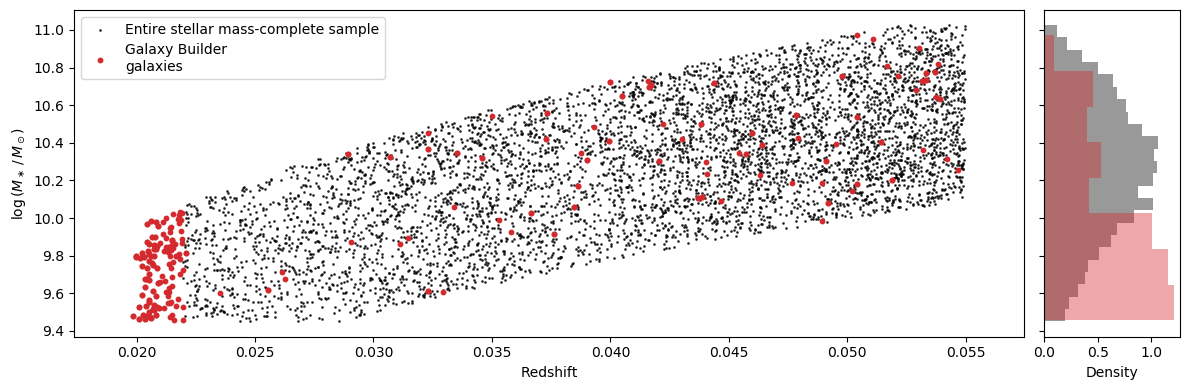
\includegraphics[width=17.7cm]{plots/stellarmass.png}
  \caption{A plot of redshift against stellar mass for the \textit{stellar mass-complete sample} from \citet{2017MNRAS.472.2263H}; the subset we use for analysis in Galaxy Builder are shown in red. At right we show a histogram of the stellar masses. This Figure is identical to Figure 4 from \citet{2020arXiv200610450L} who use the same sample.}
  \label{fig:stellarmass}
\end{figure*}

Some galaxies in \citet{2020arXiv200610450L} were shown to volunteers a second time in a repeat validation subset to create a second aggregate model used to test internal consistency. Section 3.2 of \citet{2020arXiv200610450L} presents a comparison if these classifications to investigate volunteer consistency. We can see that arm number is highly reliable within $\pm1$ (93\% galaxies have arm number counts which agree in this range; 53\% have exactly identical arm number counts). In this work, we combine the 30 classifications of galaxies in this validation subset with the 30 original classifications. Clustering of drawn spiral arms and cleaning of points was then performed as detailed in \citet{2020arXiv200610450L}. We remove any galaxies for which no spiral arms were identified, resulting in a hierarchical data structure of 129 galaxies, 247 spiral arms and 238,433 points. This breaks down further to 68 galaxies (53\% of the sample) having two arms identified (meaning that they were marked by enough users to cluster into an arm), 19 (15\%) with three such arms, 4 (3\%) with four, and the remainder (38 or 29\%) with a single identified arm. We believe that our reported number of arms per galaxy is in many cases an underestimate, and since the most common number of arms is two, this most often results in a single arm being measured when two are present. The most common way we miss an arm is if the clustering did not converge when users have appeared to identify a second arm.
For example, we find by visual inspection that just three galaxies in the sample are truly one-armed spirals, while in the remaining 35 galaxies for which only one arm was identified following clustering, the other arms were simply not recovered due to noise in the dataset. Given this, we do not recommend using these statistics to make general conclusions about the number of arms per galaxy. However, as our hierarchical model incorporates the uncertainty involved with missing spiral arms, the results related to pitch angle should not be significantly affected.

Spiral arm points are deprojected to a face-on orientation using the disk inclination and position angle obtained through photometric model fitting performed in \citet{2020arXiv200610450L}. Arms are individually corrected to all have the same chirality (a pitch angle greater than or equal to zero) using the logarithmic spiral fit in \citet{2020arXiv200610450L}. This was achieved by multiplying the polar coordinate $\theta$ by $-1$ for arms identified as winding counter-clockwise.

\subsection{Bayesian modelling of spiral arms in \textit{Galaxy Builder}}
\label{section:bhsm-model}
In this section, we lay out our Bayesian hierarchical model for galaxy pitch angle. We fit directly to clustered, cleaned points from polylines drawn in \textit{Galaxy Builder}, deprojected and unwrapped to polar coordinates. We fit a logarithmic spiral to each clustered arm (examples are shown in Figure \ref{fig:example-spiral-fits}), with the pitch angles of multiple arms in a single galaxy being drawn from a single parent distribution.

Logarithmic spirals have the desirable properties of a constant pitch angle and a small number of free parameters. For this first analysis of the \textit{Galaxy Builder} models we choose to make use of it here without an explicit comparison to other models. A simple visual inspection of the fitted logarithmic spirals suggests that it is an appropriate model, however, a comparison of a logarithmic spiral profile to other spiral forms (i.e. Archimedean or polynomial) is another important piece of work, outside of the scope of this research, as it has been reported that galaxy arms do not have constant pitch angles (\citealt{1981AJ.....86.1847K}; \citealt{2009MNRAS.397..164R}).

As suggested by spiral formation models which correlate a galaxy wide pitch angle with galaxy wide properties, we will assume that a given galaxy has some preferred value for arm pitch angle, $\phi_\mathrm{gal}$, and that the pitch angles of spiral arms in that galaxy, $\phi_\mathrm{arm}$, are constant with radius (giving logarithmic spirals) and drawn from a normal distribution centred on $\phi_\mathrm{gal}$, with some spread $\sigma_\mathrm{gal}$ common to all galaxies. We truncate the normal distribution of spiral arm pitch angles in a single galaxy between the physical limits of {0\degree} (a ring) and {90\degree} (a ``spoke''), giving

\begin{equation}
\phi_\mathrm{arm} \sim \mathrm{TruncatedNormal}(\phi_\mathrm{gal}, \sigma_\mathrm{gal}, \mathrm{min}=0, \mathrm{max}=90).
\end{equation}

The choice to assume all galaxies show the same inter-arm variation in pitch angle (represented by a common value of $\sigma_\mathrm{gal}$ across all galaxies) was motivated by our small sample size and the low number of arms measured per galaxy. With this sample size we do not find, nor expect to be sensitive to variations in this parameter. It is possible that it does vary between galaxies, and that this variation is physically interesting. Several authors have previously made attempts to measure this parameter.  In a seminal work, \citet{1981AJ.....86.1847K} fit logarithmic spirals to 113 nearby (NGC) galaxies, and note the dominant error in average galaxy pitch angle comes from inter-arm variation, which they measure to have an average value of 5$^\circ$. \citet{2014ApJ...790...87D} is primarily a machine learning method paper, and while details on the galaxies investigated are not clear, their Table 1 presents the median difference in pitch angle between pairs of arms with different lengths, which varies from 14.5$^\circ$ in very short arms, to 2.6$^\circ$ in the longest traced arms. It is unclear how much this encodes error in their method versus real variation in the galaxy population. Within our own Milky Way, \citet{Vallee2015} did a meta analysis and comparison of several technique to conclude a range of 12-14$^\circ$ (i.e. 2$^\circ$) was reasonable for all Milky Way spiral arms. In a very detailed study of four very nearby spirals, \citet{HonigRead2015} conclude there are large variations of pitch angles  between spirals, and among arms in a given spiral, but made no comments as to if the variation was consistent with being constant. Further investigation of this issue in a larger \textit{Galaxy Builder} sample would be an interesting follow-up project.

We assume that the observed points in a \textit{Galaxy Builder} spiral arm, once deprojected, follow a logarithmic spiral with gaussian radial error $\sigma_r$,

\begin{equation}
\widetilde{r_\mathrm{arm}} = \exp\left(\widevec{\theta_\mathrm{arm}}\tan\phi_\mathrm{arm} + c_\mathrm{arm}\right).
\end{equation}

Where $\widetilde{r_\mathrm{arm}}$ is the model's prediction for the radii of the deprojected points in a \textit{Galaxy Builder} arm ($\widevec{r_\mathrm{arm}}$), $c_\mathrm{arm}$ is the amplitude parameter (equivalent to $A$ in Equation \ref{eq:log-spiral}), and $\widevec{\theta_\mathrm{arm}}$ is the polar angles of the points.

We choose hyperpriors over $\phi_\mathrm{gal}$, $\sigma_\mathrm{gal}$, $c_\mathrm{arm}$ and $\sigma_\mathrm{r}$ of

\begin{align}
  \phi_\mathrm{gal} &\sim \mathrm{Uniform}(\mathrm{min}=0, \mathrm{max}=90),\\
  \sigma_\mathrm{gal} &\sim \mathrm{InverseGamma}(\alpha=2,\,\beta=20),\\
  c_\mathrm{arm} &\sim \mathrm{Cauchy}(\alpha=0,\,\beta=10),\\
  \sigma_r &\sim \mathrm{InverseGamma}(\alpha=2, \beta=0.5).
\end{align}

These are conservative priors, which are not expected to have significant impact on the results. The inverse gamma distribution is used to aid the convergence of the Hamiltonian Monte Carlo (HMC) algorithm used (discussed later). The Cauchy distribution is equivalent to the Student's t-distribution with one degree of freedom, and was chosen due to its fatter tails than the normal distribution. Our likelihood function for $N$ arms, each with $n_\mathrm{arm}$ points, is

\begin{equation}
  \mathcal{L} = \prod_{\mathrm{arm}=1}^{N}\left(2\pi\sigma_r^2\right)^{-n_\mathrm{arm}/2}
  \exp\left(-\frac{||\widevec{r_\mathrm{arm}}\,-\,\widetilde{r_\mathrm{arm}}||^2}{2\sigma_r^2}\right).
\end{equation}

We assume that the radial error is Gaussian for simplicity of analysis, however, Shapiro-Wilk tests on the residuals of the logarithmic spirals fit in \citet{2020arXiv200610450L} suggest that this is not a good assumption, and a more robust likelihood (such as the Student's t-distribution) would possibly more appropriate.

To perform inference, we make use of the No-U-Turn-Sampler (NUTS, \citealt{2011arXiv1111.4246H}), implemented in PYMC3\footnote{\url{https://docs.pymc.io/}}, an open-source probabilistic programming framework written in Python \citep{pymc3_paper}. To aid the convergence of MC chains, we scale the radii of deprojected points to have unit variance.

% \newpage

\section{Results}
% !TEX root = ../main.tex
\subsection{Constraints on Galaxy Pitch angle}
Our hierarchical model can predict individual arm pitch angle with a hich degree of certainty, however it returns a large spread of potential values for the pitch angles of arms

\subsection{Spiral Winding}
\label{section:spiral_winding}
In order to test the possible progenitor distribution of our estimated galaxy pitch angles, we repeatedly perform an Anderson-Darling test over each draw present in the MCMC trace, resulting in a distribution of Anderson-Darling statistics. We will refer to this test as the \textit{marginalized Anderson-Darling test}. We make use of the Kolmogorov-Smirnov test in a similar manner for comparison.

We perform the marginalized Anderson-Darling test for a potential source distribution uniform in $\cot\phi$ between the limits present in \citet{2019arXiv190910291P} ($1.00 < \cot\phi < 4.75$, or roughly $11.9^\circ < \phi < 45.0^\circ$). The resulting distribution of Anderson-Darling statistics can be seen in Figure \ref{fig:ad-cot-test}. We observe that we reject the null hypothesis at the 1\% level for only 86\% of the possible realizations of galaxy pitch angle, therefore with our sample and methodology we cannot unilaterally reject winding of the kind described by \citet{2019arXiv190910291P}.

\begin{figure*}
  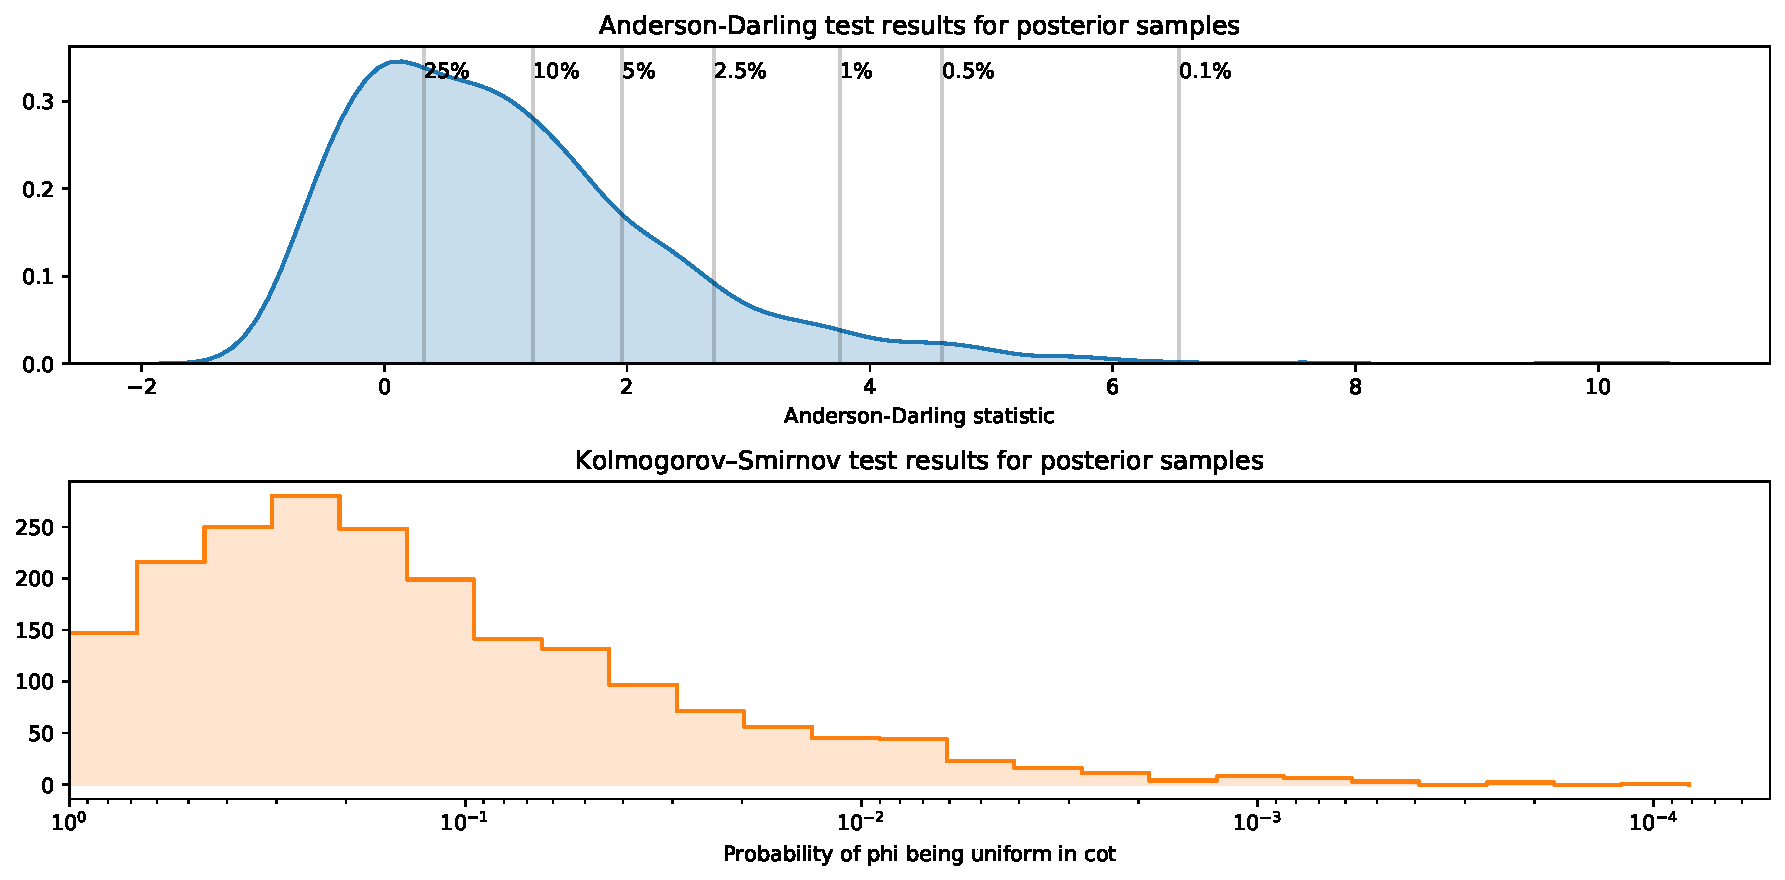
\includegraphics[width=17.7cm]{plots/cot_uniform_marginalized_tests.pdf}
  \caption{The results of a marginalized Anderson-Darling test (top panel), with values corresponding to various confidence intervals shown, and marginalized Kolmogorov-Smirnov test p-values (lower panel). Moving rightwards on the x-axis implies greater confidence in rejecting the null hypothesis.}
  \label{fig:ad-cot-test}
\end{figure*}

\subsection{Dependence of pitch angle on Galaxy Morphology}
\label{section:morphology_comparision}
\subsubsection{Pitch angle vs. Bulge size}
We see no correlation between galaxy pitch angle derived from the \textit{hierarchical normal model} and Galaxy Zoo 2's debiased \citep{Willett2013:1308.3496v2} \textit{pbulge}, which has been shown to be a good measure of bulge size.

We separate our sample into ``disc-dominated galaxies'' and ``obvious bulge galaxies'' using the debiased fractions from Galaxy Zoo 2 following \citet{2017MNRAS.469.3363K}, defining \textit{no bulge + just noticeable $>$ obvious + dominant} for the former and the converse for the latter. A marginalized two-sample Anderson-Darling test \citep{doi:10.1080/01621459.1987.10478517} does not find strong evidence that the samples were drawn from different distributions; we reject the null hypothesis at the 1\% level for only 8\% of the samples.


\subsubsection{Pitch angle vs. Bar Strength}
We see no correlation between galaxy pitch angle derived from the \textit{hierarchical normal model} and Galaxy Zoo 2's debiased \textit{pbar}, which is widely viewed as a good measure of bar strength, and therefore a measure of the torque applied on the disc gas.

Separating the sample based off of $\mathrm{\textit{pbar}} > 0.5$, and restricting to galaxies with more than 10 classifications for \textit{pbar} (as performed by \citealt{2011MNRAS.411.2026M} and \citealt{2017MNRAS.469.3363K}) and performing a marginalized two-sample Anderson-Darling test does not find that the samples were drawn from different distributions. \comment{Talk about number of galaxies in each sub-sample?}


\begin{figure*}
  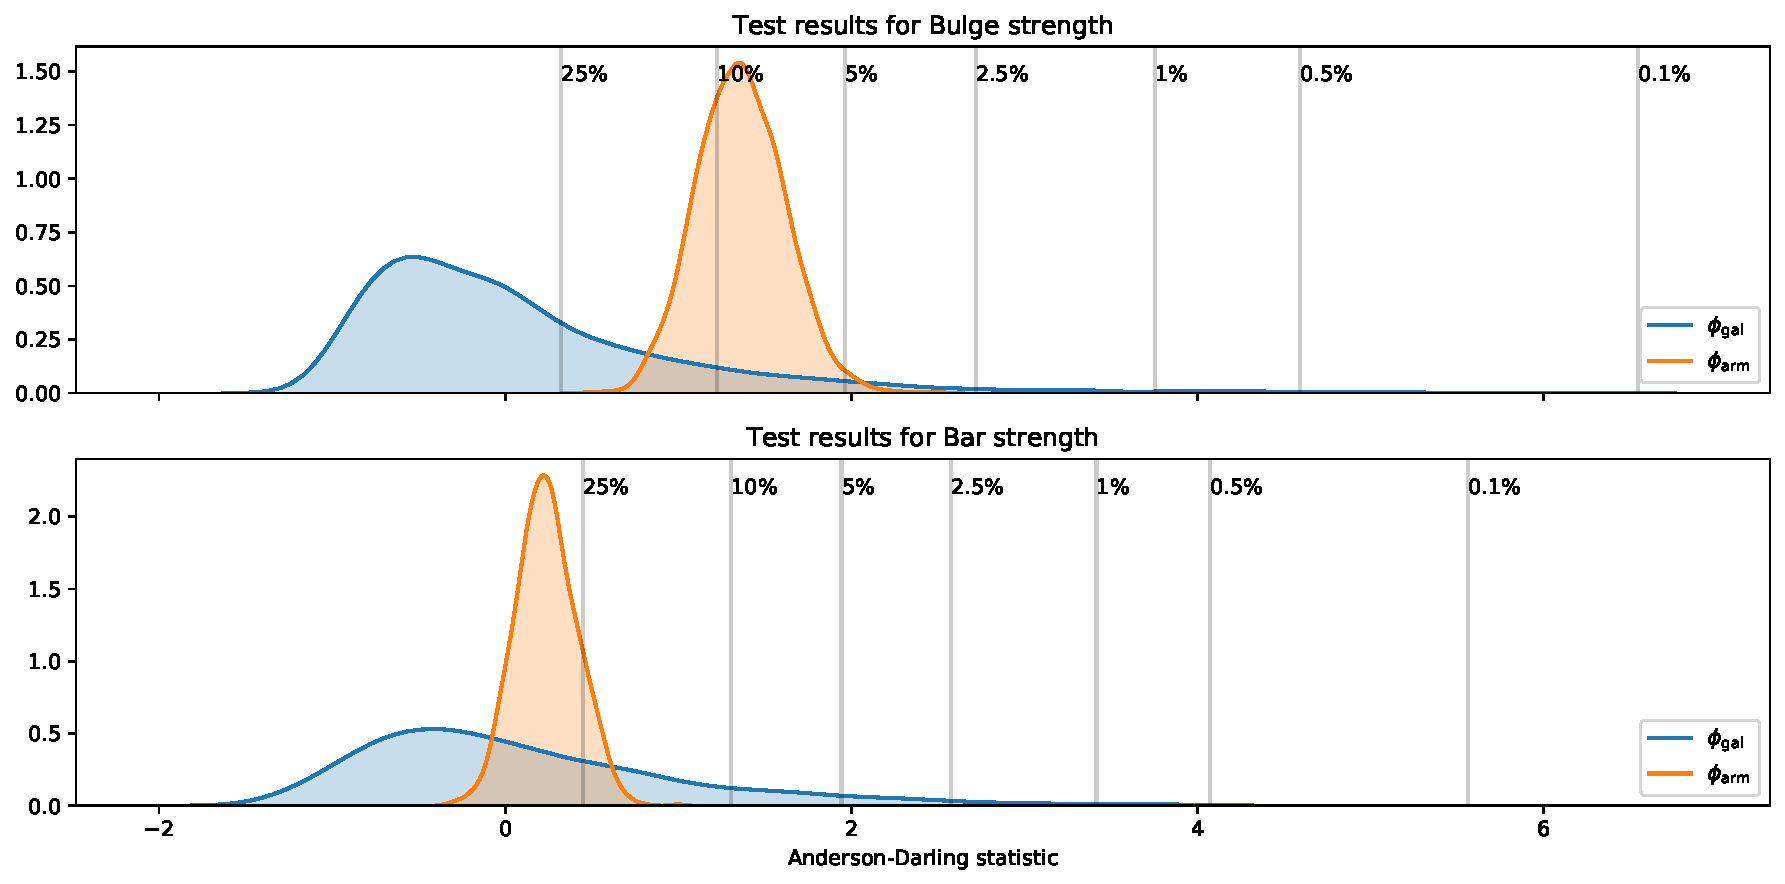
\includegraphics[width=17.7cm]{plots/bulge_bar_test_results.pdf}
  \caption{The results of marginalized two-sample Anderson-Darling tests examining whether pitch angles for Bulge-dominated and Disc-dominated galaxies are drawn from the same distribution (top panel), and the results of the same test for strongly-barred vs unbarred galaxies (bottom panel).}
  \label{fig:ad-morphology-test}
\end{figure*}

% \newpage

\section{Discussion and Conclusions}
% !TEX root = ../main.tex
This paper presents a new Bayesian approach to estimate galaxy pitch angle, making use of citizen science results to measure spiral arms through photometric modelling. We introduce an adaptation of the Anderson-Darling test, which we name the \textit{marginalized Anderson-Darling test}, to incorporate full Bayesian posterior probabilities and utilize this test to investigate theories governing spiral formation and evolution.

The statistical approach implemented in this paper allows a more thorough examination of pitch angle than length-weighted pitch angle calculation, and better accounts for the large varitations observed in inter-arm pitch angle than fourier analysis, which assumes all arms in a given mode have the same pitch angle.

We do not see a relationship between bar strength and pitch angle in our data, as would have been predicted by Manifold theory, and do not find evidence for the relationship between bulge size and pitch angle predicted by the Hubble sequence. \citet{2007ApJ...655...77G} propose that bulge S\'ersic index is correlated with black hole mass, which has in turn been shown to correlate with spiral pitch angle, we do not investigate this here as \textit{Galaxy Builder} could not accurately recover bulge S\'ersic indices.

Our results are consistent with spiral winding of the form described by \citet{2019arXiv190910291P}, in which spiral arms are transient and reccurent, evolve through mechanisms such as swing-amplification \citep{1965MNRAS.130..125G} and which wind up over time. However, the assumptions of this model of spiral winding are highly simplistic, and it leaves many unanswered questions: what determines the limits on $\phi$? Is the spiral arm equally apparent at all pitch angles, or is a selection effect present? This result is also not evidence against QSDW, as it is possible that our distribtuion of pitch angles is dictated by other factors such as disk shear and central mass concentration.

We do not account for observation effects, instead assuming that galaxy builder spiral arms are equally likely to be identified and recovered at all pitch angles within the limits specified above. We also assume that the galaxy sample is representative of the general spiral population, which is not necessarily the case. As with most analyses, the most impactful improvement it would be possible to make here would be to increase the cleanliness and volume of data analysed; due to time constraints the \textit{Galaxy Builder} galaxies used are not guaranteed to be representative.

The methodlogy proposed here is a robust solution to the problems facing investigation of spiral morphology, namely that of reliably identifying spiral arms, and properly accounting for the spread in pitch angles of arms within a galaxy.

% \newpage

\section{Acknowledgements}
% !TEX root = ../main.tex
This publication made use of SDSS-I/II data. Funding for the SDSS and SDSS-II was provided by the Alfred P. Sloan Foundation, the Participating Institutions, the National Science Foundation, the U.S. Department of Energy, the National Aeronautics and Space Administration, the Japanese Monbukagakusho, the Max Planck Society, and the Higher Education Funding Council for England. The SDSS Web Site is \url{http://www.sdss.org/}.

This project was partially funded by a Google Faculty Research Award to Karen Masters (\url{https://ai.google/research/outreach/faculty-research-awards/})

% \newpage

%%%%%%%%%%%%%%%%%%%%%%%%%%%%%%%%%%%%%%%%%%%%%%%%%%

%%%%%%%%%%%%%%%%%%%% REFERENCES %%%%%%%%%%%%%%%%%%

% The best way to enter references is to use BibTeX:
\bibliographystyle{mnras}
\bibliography{bibliography} % if your bibtex file is called example.bib

%%%%%%%%%%%%%%%%%%%%%%%%%%%%%%%%%%%%%%%%%%%%%%%%%%

%%%%%%%%%%%%%%%%% APPENDICES %%%%%%%%%%%%%%%%%%%%%

\appendix

\subfile{sections/appendix}

%%%%%%%%%%%%%%%%%%%%%%%%%%%%%%%%%%%%%%%%%%%%%%%%%%


% Don't change these lines
\bsp	% typesetting comment
\label{lastpage}
\end{document}

% End of mnras_template.tex
